\section{Introducción}
\subsubsection{Preámbulo}

Los asistentes virtuales cada vez están más presentes en nuestras vidas gracias a todos los avances de la tecnología, y puede verse en que ya aparecen en todos los teléfonos móviles para ayudar en el día a día de los usuarios, ya sea para responder preguntas, poner una canción, o buscar información de manera rápida para el usuario.

La utilización de estos asistentes virtuales hace que cada vez más personas se planteen la posibilidad de llevar más lejos la utilización de ellos, como puede ser a través de otros dispositivos inteligentes a los que se les está buscando hueco cada vez en más hogares.

Estos dispositivos nos hacen la vida más sencilla, ayudando a actualizar y controlar toda la domótica de nuestras casas, de manera que se puedan realizar acciones en nuestra vivienda que hace unos años solo se podían imaginar en películas de ciencia ficción.

La utilización de asistentes virtuales para facilitar acciones que se repiten de manera continuada a lo largo de los días está cada vez más de moda: según un estudio de la reputada Nielsen~\cite{nielsen}, durante el Q2 de 2018 ha llegado a crecer el número de dispositivos desplegados en los hogares de Estados Unidos hasta alcanzar el 24\% de la población.

A la pregunta de para qué puede querer el 24\% de las familias un dispositivo asistente en sus casas, se puede observar tras una encuesta de dicho estudio, que en la mayoría de hogares se daba un uso bastante simple, solicitando al dispositivo únicamente la reproducción de contenido multimedia, pero esto ocurre únicamente en las primeras semanas de uso. También se puede observar en el estudio que, posteriormente, se tiende a dar más uso al dispositivo llegándole a requerir información habitual que se requiere de manera repetitiva cada semana, como puede ser la consulta del tiempo, la del tráfico antes de ir a trabajar o a la consulta de algún evento cercano importante.

La simplicidad de uso y todas las posibilidades que abarca ha hecho que una vez ha sido usado este tipo de dispositivo inteligente en cualquier hogar, se le siga utilizando cada vez para más tareas, dada su usabilidad y abanico de utilidades.

En ese estudio arriba citado, también se puede observar el comportamiento de los usuarios: una vez el dispositivo está en entre las cuatro paredes de la casa, se tiende a acompañar a este dispositivo inteligente de otros dispositivos domóticos, convirtiendo poco a poco el hogar en un sistema interconectado: cuatro de cada diez hogares disponen de más de un dispositivo inteligente en el hogar, y el 45\% de los hogares se plantean acompañar al que ya tienen, comprando otro.

Esta gran aceptación a la domótica viene dada gracias a la cantidad de variantes de las cuales podemos dotar al hogar, pudiendo ser todas controladas a través del dispositivo asistente, así como puede ser la programación de los tiempos de uso de aparatos como las bombillas, el termostato, los sistemas de seguridad, e incluso tanto el frigorífico, el sistema de riego, u otras acciones relativas a la seguridad de la vivienda como puede ser bloquear las puertas y ventanas, al igual que mantener el registro de cuáles y cuándo han sido abiertas, entre otras muchas opciones.

Al irrumpir estos dispositivos en las acciones cotidianas de un día corriente, se le permite al usuario adaptarse y ver que estos aparatos le acaban facilitando el día.

Viendo el creciente uso de estos dispositivos y las grandes marcas que hacen acto de presencia facilitando su implementación, entre las cuales se encuentran Google o Amazon, se puede pensar que este mercado ya está dominado y pertenece a estos dos grandes imperios, pero en este caso no se va a tener en cuenta todo lo que ya ofrecen, sino que se va a tener en cuenta todo lo que no están ofreciendo, o qué es lo que sus dispositivos no están preparados para ofrecer:

Como bien se ha visto, el punto de mira en todo el tema de la domótica y asistentes tiene un público objetivo que es el que pertenece a un rango de edad al que le gusta la tecnología y le parecería interesante automatizar las tareas del hogar, pero el verdadero público que podría exprimir todo su potencial es el público que menos acostumbrado nos tiene a estar a la vanguardia de la tecnología, el público perteneciente a la tercera edad.

Si se realiza el acto de volver a pensar sobre lo que es un asistente personal, en cuanto a una persona que trabaja como asistente, se entiende que es una persona que ayuda en las acciones del día a día más simples y repetitivas para las que otra persona no es capaz de hacer por si misma por algún tipo de incapacidad, ya sea incapacidad temporal, o algún tipo de incapacidad física.

Una vez planteado a qué se dedica un asistente personal, es fácil darse cuenta que al hablar de este trabajador se plasme la imagen de una persona que ayuda a personas mayores, o a personas con algún tipo de discapacidad.

El rango de personas de tercera edad es un público que puede necesitar que le levanten las persianas de manera automática porque quizá, le cuesta levantarse de la cama. Es un público que puede necesitar utilizar un asistente que le recuerde realizar ciertas tareas en su día a día como puede ser ir al médico, tomarse la pastilla, hacer la compra, o recordarle qué productos tiene que comprar, al igual que el cumpleaños de un ser querido. Todo esto acompañado de la seguridad que le puede proporcionar tareas como asegurarse que todas las puertas de su casa están bien cerradas, o saber que aún estando estas personas solas en casa, podrían solicitar auxilio en un momento de urgencia a través del asistente.

La tecnología vinculada a Internet nos hace la vida más sencilla a través del smartphone o de los ordenadores, pero las labores que nos proporciona como extra un dispositivo asistente inteligente a un usuario medio el cual ya está acostumbrado a usar un smartphone son muy pocas, ya que podría realizarlas a través de su propio teléfono, en cambio, a una persona de tercera edad a la cual le cuesta hacer un uso normal de dispositivos tecnológicos, un dispositivo asistente inteligente podría hacerle la vida mucho más sencilla, ya que lo único que necesitaría sería establecer una conversación oral con el dispositivo, evitando el intermediario que supone un ordenador o un smartphone.

El rango de personas de tercera edad, es por tanto el público que más puede necesitar un dispositivo asistente, así como el público que más puede llegar a exprimirlo.

La creación de un asistente que pueda resolver sus dudas, con el que pueda hablar, al que pueda preguntar a qué hora es la partida de cartas en el bar, o al que puedan pedir auxilio en caso de una caída, puede ser de gran utilidad para mejorar su día a día, al igual que servir de alivio para el resto de familiares que no pueden estar cerca de sus seres queridos, sabiendo que van a poder ser informados rápidamente de un posible accidente.

He aquí, por tanto, el agujero de mercado que ha sido encontrado en las grandes empresas antes nombradas, y el cual puede permitir un modelo de negocio el cual tenga como premisa buscar la satisfacción de las personas mayores, que igualmente puede servir para dar libertad a otros grupos sociales, como pueden ser las personas con algún tipo de discapacidad.

El auge de los dispositivos asistentes se puede ver como una evolución tecnológica que permita facilitar las rutinas, pero también con ello se pone en vilo la gestión de la privacidad e intimidad que hay dentro de nuestras casas. Esto es debido a que este tipo de dispositivos inteligentes pueden recolectar información a través de escuchar las conversaciones de un usuario y su día a día, siendo información que no se sabe de manera exacta a dónde va a parar, o qué se va a hacer con ella.

Esta información captada puede ser de un carácter sensible, ya que puede contener desde simples gustos, incluyendo las necesidades del usuario, como sus tendencias políticas, siendo datos que pueden estar siendo utilizados por terceros, o incluso pudiendo estar siendo vendidos.

La falta de soluciones en el mercado que cumplan todos estos puntos supone una motivación para la creación de un asistente que no esté conectado constantemente a Internet, ya que las personas de edad avanzada seguramente no tengan contratado el servicio, y que tampoco almacene datos de carácter sensible de los usuarios, sino que simplemente interaccione con cada persona y la ayude en su día a día, tanto ofreciendo actividades de la misma localidad, como respondiendo cualquier pregunta que pase por la cabeza de quien lo posea, al igual que buscando ayuda en caso de que una persona requiera auxilio.

Antes de adentrar en la elección de un asistente inteligente, se expondrá qué es, y cuál es su funcionamiento, para entender mejor los motivos por los cuales se acaba eligiendo uno en vez de otro.

\subsubsection{Qué es un Asistente Inteligente}

Un asistente inteligente es una máquina programada de tal manera que su comportamiento se asemeje al de una persona a la que se solicita asistencia, como su propio nombre indica, pudiendo mantener una conversación que siga los protocolos de comunicación humana.

\begin{figure}[h!]
    \centering
    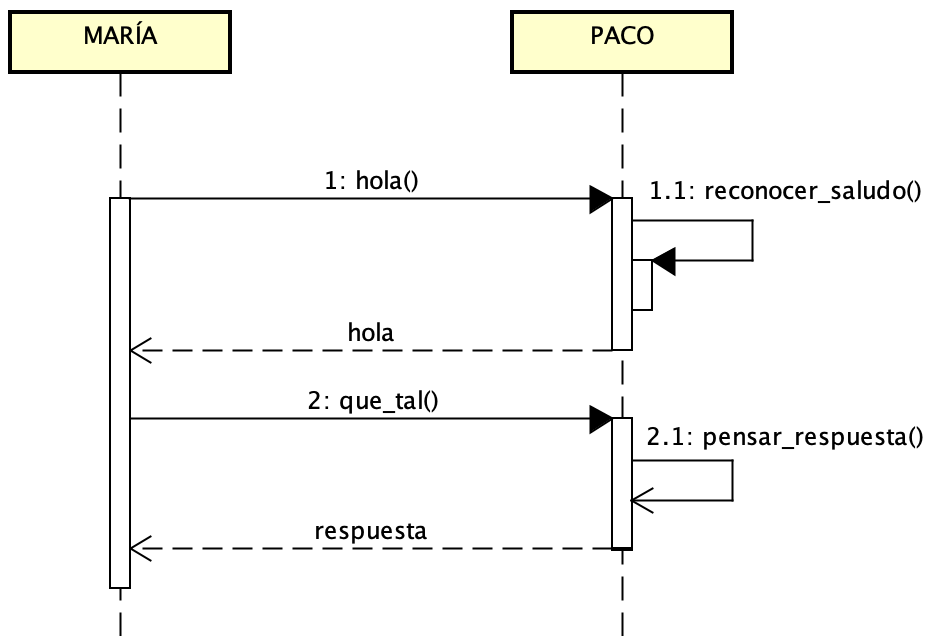
\includegraphics[width=10cm]{./img/sequence/human.png}
    \caption{Secuencia de Comunicación humana}
    \label{fig:humanseq}
\end{figure}

Como se puede ver en la figura \ref{fig:humanseq}, un protocolo de comunicación entre dos personas se basaría en un saludo para entablar conversación, para posteriormente realizar una pregunta.

En el caso de los asistentes, el proceso de conversación se basa en lo mismo: un usuario saluda al asistente mediante el uso de una palabra o conjunto de palabras, al que se llamará \textbf{hotword}, que cuando sea reconocido por el asistente inteligente, devolverá el saludo.
Es entonces cuando el usuario debe realizar la pregunta o solicitar la información que requiera.
Una vez hecha la pregunta, el dispositivo se pondrá a pensar la posible respuesta, entrando en el proceso al que se llamará \textbf{reconocimiento de los hechos}. Una vez identificados los hechos, devolverá la respuesta que más se acerque a lo deseado, gracias a un entrenamiento previo.

\newpage
\subsubsection{Cómo Piensa el Asistente}

El proceso de pensamiento analizado de los principales asistentes del mercado, que se expondrá en el presente capítulo, tiene una estructura similar independientemente del tipo de asistente que se trate, asemejándose a la figura \ref{fig:humasseq}.

\begin{figure}[h!]
    \centering
    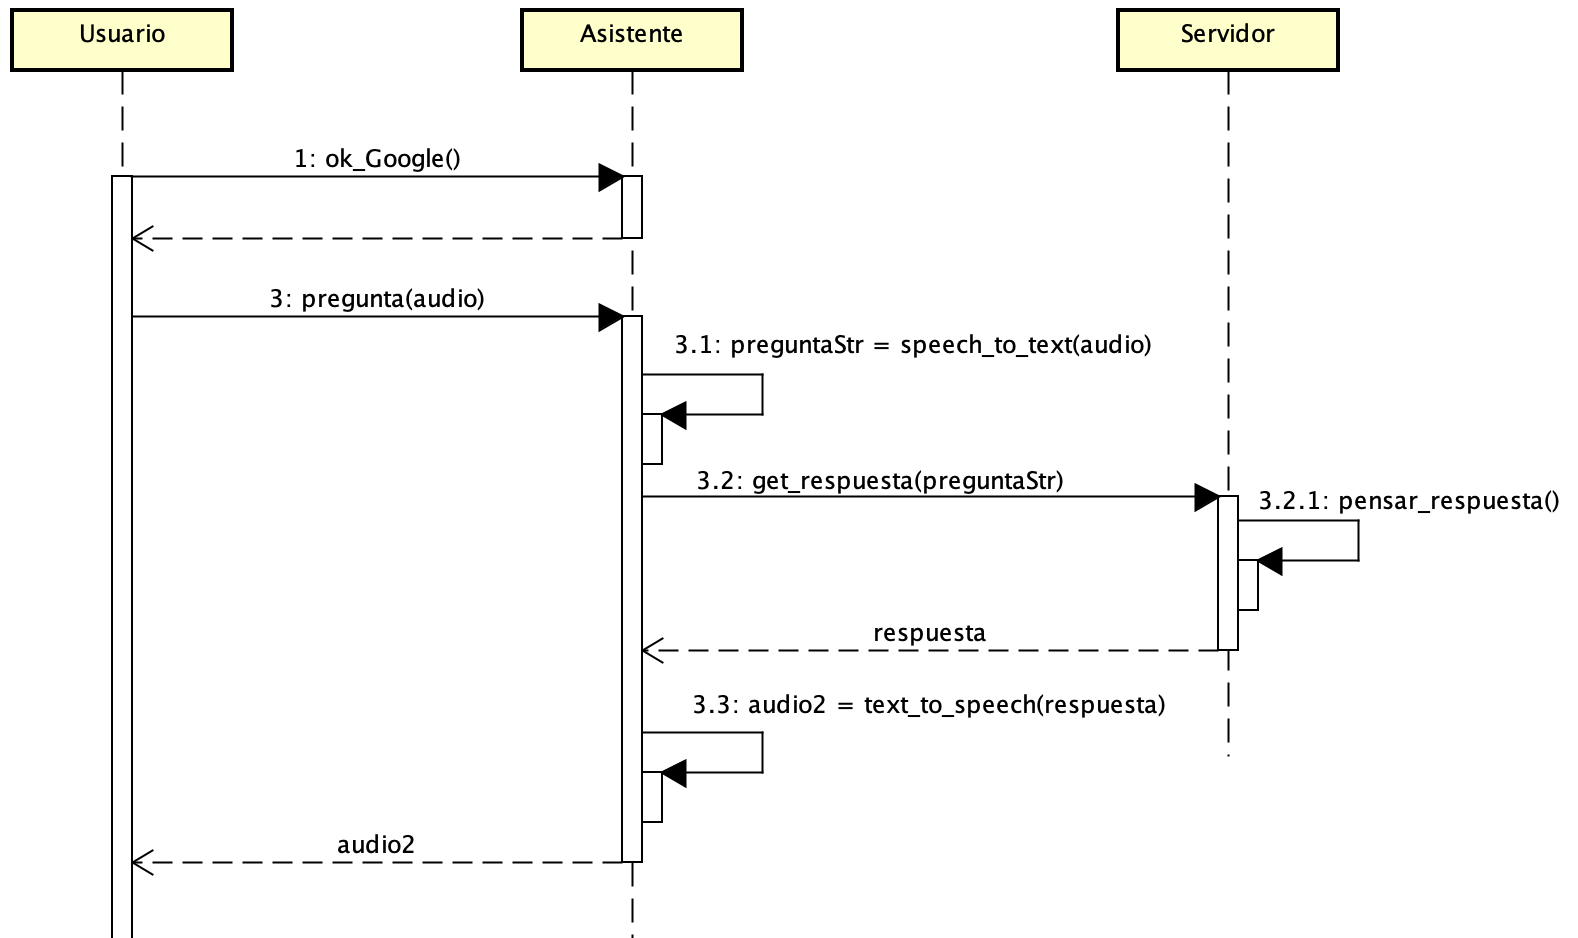
\includegraphics[width=13cm]{./img/sequence/humasseq.png}
    \caption{Secuencia de Comunicación humano-asistente}
    \label{fig:humasseq}
\end{figure}

Lo que diferencia a un asistente de otro, es la manera en la cual piensa la respuesta, dando mayor validez a un asistente que dé una respuesta más aproximada a lo solicitado.
Para lograr dar la respuesta más acertada, la mayoría de los asistentes existentes realizan el procesamiento de la respuesta en la nube debido a la gran cantidad de información que tienen previamente almacenada de otras consulta de otros usuarios para contrastar los hechos capturados, al igual que también pueden realizar en la nube el proceso de speech-to-text enviando los audios a sus servidores y transformándolo ahí a cadenas de texto, o el de text-to-speech, que sería el proceso inverso.


\section{Requisitos mínimos}
Una vez que ya se ha expuesto cual es el funcionamiento base de un asistente virtual inteligente, interesa saber cuál es de todos los existentes que más se adecúa a las necesidades establecidas para este proyecto, de manera que se le exijirá que cumpla el máximo de los siguientes puntos expuestos.

\subsubsection{Despliegue en Dispositivos}

El asistente seleccionado debe poder ser desplegado de manera gratuíta en un dispositivo formado por una placa RasbperryPi, o similar.

Para ello, se requiere que el asistente disponga de una librería o de un modo de uso que se pueda implementar en un dispositivo pequeño y portátil, facilitando el cambio de una ubicación física por otra de los distintos posibles puntos que existen dentro de un hogar, manteniendo una instalación lo más simple y limpia posible, en la que solo sea requerida la localización de un enchufe activo que posea corriente eléctrica.

\subsubsection{Tratamiento de la Información}

El asistente debe seguir la Ley Orgánica de Protección de Datos~\cite{lopd}, y no debe tener acceso a escuchar conversaciones ajenas violando la intimidad de los usuarios.

Cualquier vacío legal o conjunto de cláusulas de extensa longitud no podrá será aceptado, para poder asegurar la protección de los datos de los usuarios.

En caso de almacenar algún tipo de dato, debe poder ser público para el usuario en cuestión, o haber sido aceptado expresamente por el usuario a favor de un control de su seguridad.

\subsubsection{Conexión a Internet}

La orientación de un dispositivo asistente inteligente como este a personas de una edad avanzada debe tener en cuenta que es posible que la mayoría de sus usuarios potenciales no tengan una conexión a internet en sus respectivos hogares.

Esto provoca que la conexión del dispositivo a la red tiene que ser lo mínima posible, favoreciendo los asistentes en los cuales el proceso de pensamiento sea ejecutado dentro del propio dispositivo, evitando tener que hacer el cálculo e identificación en servidores de alojados en la nube.

Es decir, el dispositivo debe ser capaz de funcionar en el lugar más remoto posible y sin ninguna conexión a internet, simplemente tras ser conectado a una red eléctrica.

\subsubsection{Adicción de Nuevas Tareas}

El software del asistente inteligente debe tener la capacidad de añadir nuevas tareas fácilmente, de modo que se puedan añadir nuevas funciones tanto propias, como desarrolladas por la comunidad de Internet.

\section{Mercado}
\label{mercato}
En los siguientes apartados se mostrarán las diferentes opciones que ofrece ya el mercado para el uso de asistentes inteligentes, con el fin de comprobar la existencia de alguno que ya tenga establecidos los requisitos base ya descritos, o que permita la opción de poder establecerlos.

    \subsection{Google Assistant}
    El asistente inteligente de Google es el que está en el año 2020 a la cabeza de los asistentes virtuales~\cite{top-asistentes}, y esto es debido a que viene instalado en todos los dispositivos Android, ocupando estos dispositivos la mayor parte del mercado de la telefonía móvil. Esta posición privilegiada le proporciona un mayor entrenamiento, dando por resultado una elevada tasa de acierto que como consecuencia le atribuye mayor usabilidad.

Esta creación de Google tiene una gran aceptación con los diferentes aparatos existentes para la domótica del hogar, facilitando la implementación y realización de tareas:

- Una tarea es un conjunto de acciones que se llevan a cabo tras accionarse un evento que hace de interruptor, pudiendo ser el evento tanto un comando de voz, la pulsación de un interruptor o la activación de un sensor, entre otras opciones.

De esta manera, Google permite el control de la domótica del hogar, o la realización de diferentes acciones en nuestro día a día, pero requiere ser configurado por cada usuario, evitando por tanto la posibilidad de un despliegue común.

\subsubsection{Cómo Funciona}

El proceso de pensamiento que hace el asistente de Google está basado en la nube, pero no solo eso sino que Google hace en sus servidores también el proceso de Speech-to-Text.

De este modo, Google almacena todos los audios\cite{google-almacena} que se le mandan a través de su asistente, estudiándolos uno a uno y asegurando o corrigiendo sobre la respuesta que envió el asistente.

Este proceso de corregir o confirmar es el método que tiene Google de entrenamiento, de manera que en la próxima consulta sobre el mismo tema, el asistente pueda responder con mayor exactitud.

Queda claro que sobre la teoría es un buen plan de entrenamiento, y en un mundo ideal esto sería perfecto, pero esos audios también pueden contener parte de información privada, o pueden servir para espiar conversaciones privadas que un usuario puede no querer que estén almacenadas, ni que sean escuchadas por otra persona, aunque sea un propio trabajador.

En cuanto a la posibilidad de ser desplegado en otro dispositivo que no sea un smartphone o una tablet, Google nos lo pone fácil, ya que otorga una librería con la cuál facilita la instalación y uso en una gran variedad de dispositivos, cuyo requisito es que dispongan de conexión a Internet.


    
    \subsection{Amazon Echo}
    ~También conocido como Alexa, es la opción creada por Amazon que más fuerza está tomando en la sociedad para ser elegida como el asistente de voz inteligente que nos acompañe en nuestro día a día.

A pesar de todas las ventajas posibles similares a las que se han descrito para el asistente de Google, también comparte sus contras, como las referentes a la localización donde se procesan los audios y donde se efectúa el entrenamiento, por lo que es otra opción que va a ser rechazada.

Sin tener en cuenta la ubicación del proceso de pensamiento, Amazon asegura\cite{escandalo-amazon} que almacena todos los audios hasta que es el propio usuario quien decide borrarlos, pero aún con la solicitud expresa del usuario no pueden ser borrados completamente ya que han sido compartidos con terceros, que son quienes han desarrollado funciones específicas, llamadas Skills. Estos desarrolladores no solo tienen acceso a los audios sino que los poseen, pudiendo hacer una mala práctica con ellos.

Por tanto, aunque el usuario en cuestión pida a Amazon el borrado de estos ficheros, la compañía únicamente podría borrar los archivos que posee, permaneciendo todos los cuales un desarrollador de estas skills haya almacenado, sin permitir que el propio Amazon sea capaz de eliminarlos aunque tratase de hacerlo.
    
    \subsection{Mycroft}\label{Microft}
    Ante la falta de privacidad por parte de Google y Amazon, se abre la puerta a Mycroft, proyecto Open Source que busca como pilar la seguridad de los datos y la protección de la privacidad, de manera que asegura no almacenar ningún dato o información del usuario potencial.~\cite{mycroft-doc}

Mycroft tiene una de las mayores comunidades OpenSource activa para el desarrollo e implementación de asistentes~\cite{mycroft-com}, de modo que dispone de una gran cantidad de skills que añadir a nuestro dispositivo, posicionándose como opción principal para la elaboración del proyecto.

Este asistente virtual puede ser fácilmente implementado en dispositivos tales como Raspberry, cumpliendo los propósitos y requisitos de este proyecto.

En cuanto a la conexión a Internet, el equipo de Mycroft informa acerca de estar trabajando en una herramienta que permita desplegar el asistente ya entrenado dentro del dispositivo, evitando la conexión, pero de momento esa herramienta no está finalizada, por lo que cojea en ese aspecto y de momento, debería tener una conexión permanente.

En caso de que estén en lo cierto y estén trabajando en esa herramienta, este asistente ocuparía la primera opción como asistente a desplegar, pero en el momento actual en el cual este proyecto cobra vida, no es viable su implementación.


    
    \subsection{Snips AI}
    Snips Seeed es una  plataforma de inteligencia artificial para el desarrollo de dispositivos asistentes.

Esta plataforma nos permite crear nuestro propio asistente basándose en un entrenamiento previo con unos hechos predefinidos por el desarrollador.

En ese entrenamiento previo, se permite al asistente tomar lo aprendido de otros skills, que son fáciles de añadir.

Tras la implementación en el dispositivo físico, el asistente ya ha sido entrenado, por lo cual no necesitaría volver a estar conectado a internet, siendo este el mayor argumento a favor ya que es la carencia del resto de asistentes.

En cuanto a su uso, el dispositivo solamente se mantiene a la espera de poder recibir el \textit{hotword}. Este hotword puede ser modificado por cualquier otra palabra que se desee, lo cual beneficia al proyecto actual con la posibilidad de asignar una palabra más acorde y familiar a las personas a quienes va orientado.

El asistente, en cuanto a su configuración interna, sigue el protocolo de comunicación descrito en la figura \ref{fig:humasseq}, con una pequeña modificación:
Cuando el servidor ya ha entendido la pregunta o solicitud, genera unos hechos definidos en su entrenamiento en forma de objeto que envía a través de un puerto MQTT, y se queda a la espera de una respuesta.

Los otros skills, que han sido añadidos previamente en el entrenamiento, están levantados escuchando por el puerto, de manera que identifican los objetos que circulan por él y comprueban si ese hecho le corresponde, que de no ser así, simplemente lo ignoran.
Una vez que un skill captura un hecho que sí que le corresponde, comprueba los \textit{slots} que contiene dicho hecho para ver qué es lo que se está solicitando. Tras esto, genera una respuesta en forma de cadena de texto, y la envía por el puerto MQTT para que la recoja el \textit{skill-server}.

Una vez capturada por este, simplemente transcribe el mensaje a audio con su skill de text-to-speech, y se lo transmite al usuario a través del altavoz, finalizando la comunicación.

Como se puede ver, el tratamiento de la información que se le otorga al dispositivo es el que nosotros deseemos, ya que el asistente no envía nada al exterior. De esta manera, nosotros controlamos qué sucede con la información, siendo el otro punto requerido en la búsqueda de un asistente ideal.

Como extra, Snips Seeed es una plataforma gratuita que se basa en una colaboración de una gran comunidad de desarrolladores. Pese a ser esta comunidad de menor tamaño que la conseguida por la opción de Mycroft, hay una gran cantidad de aplicaciones disponibles como juegos, la consulta del tiempo o la consulta de noticias, preparadas para ser asignadas directamente a nuestro dispositivo.

Como se puede ver, SnipsSeeed otorga las herramientas necesarias para cumplir todos los requisitos estipulados anteriormente, siendo la plataforma que se pone a la cabeza como posible elección.

    
    \subsection{Elección Final}

La elección más acorde de entre todas las propuestas es el uso Snips AI, ya que se adapta a todos nuestros requisitos.

En cuanto al proyecto, va a ser necesario el desarrollo de un dispositivo que contenga este asistente, al igual que el diseño y desarrollo de un backend capaz de albergar la información relativa a cada dispositivo.

Para la gestión de estos dispositivos también será necesaria la implementación de una página web, desde la cual puedan ser los dispositivos configurados, manejados y controlados.

La implementación operativa de todo este sistema formaría un proyecto de gran embergadura, por lo que en los siguientes capitulos se documentará el diseño y desarrollo del backend y del frontend, mostrando el control y gestión real de un dispositivo el cual su rango de funciones será breve, de modo que se establezca la base y se explique como puedan ser añadidas nuevas funciones de una manera simple y sencilla.
